
%% jan. 4, 2011  items to fix:
%% notation for math and reference to images.
%% how include eps figures.
%% make all the little figures (search for eps) in a common, nice matlab way for the
%% example filtering operations.

%\setcounter{chapter}{22}
\chapter{Temporal filters}
\label{chapter:temporal_filters}

%\section{Temporal convolutional filters}


Although adding time might seem like a trivial extension from 2D signals to 3D signals, and in many aspects it is, there are some properties of how the world behaves that make sequences to be different from arbitrary 3D signals. In 2D images most objects are bounded occupying compact and well defined image regions. However, in sequences, objects do not appear and disappear instantaneously unless they get occluded behind other objects or enter or exit the scene through doors or the image boundaries. So, the behavior of objects across time $t$ is very different than their behavior across space $n,m$. In time, objects move and deform defining continuous trajectories that have no beginning and never end. 



\section{Modeling sequences}
\label{sect:modelingSequences}

Sequences will be represented as functions $f (x,y,t)$, where $x,y$ are the spatial coordinates and $t$ is time. As before, when processing sequences we will work with the discretized version that we will represent as $f \left[n,m,t \right]$, where $n,m$ are the pixel indices and $t$ is the frame number. Discrete sequences will be bounded in space and time, and can be stored as arrays of size $N \times M \times P$.


\begin{figure}
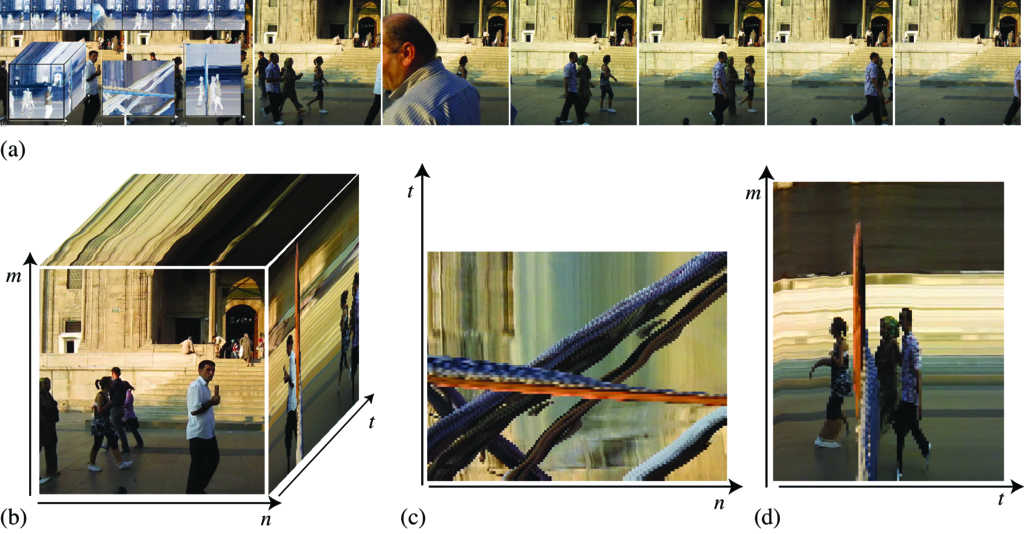
\includegraphics[width=1\linewidth]{figures/temporal_filters/motion_illustration.eps}
\caption{a) 8 Frames from a sequence with people walking. The frames are shown at regular time intervals. The full sequence had 90 frames (corresponding to 3 seconds of video). b) Space-time array, $f \left[n,m,t \right]$ of size $128 \times 128 \times 90$. c) Section for $m=50$, d) Section for $n=75$. Static objects appear as straight lines.} 
\label{fig:motion}
\end{figure}

Figure~\ref{fig:motion} illustrates this with one sequence shown in fig.~\ref{fig:motion}.a. This sequence has 90 frames and shows people on the street walking parallel to the camera plane and at different distances from the camera. Fig.~\ref{fig:motion}.b shows the space-time array $f \left[n,m,t \right]$. When we look at a picture we are a looking at a 2D section, $t=constant$, of this cube. But it is interesting to look at sections along other orientations.  Fig.~\ref{fig:motion}.c and d show sections for $m=constant$ and $n=constant$ respectively. Although they are also 2D images, their structure looks very different from the images we are used to seeing. Fig.~\ref{fig:motion}.c shows an horizontal section that is parallel to the direction of motion of the people walking. Here we see straight bands with different orientations. This bands appear to occlude each other. Each band corresponds to one person and its orientation is given by the speed of walk and the direction of motion. Fig.~\ref{fig:motion}.d looks like a foto-finish photograph as the ones used in sporting races. In both images (d) and (c), static objects appear as vertical stripes in (b), and horizontal stripes in (d). 

One special sequence is when the image has a global motion with constant velocity $(v_x,v_y)$. In such a case we can write:
\begin{equation}
f (x,y,t) = f_0 (x-v_xt,y-v_yt)
\end{equation}
where $f_0(x,y)= f (x,y,0)$ is the image being translated, and $v_x$ and $v_y$ are constants. We use continuous functions because it allows us to deal with any velocity values. This function assumes also that the brightness of the pixels does not change while the scene is moving ({\bf constant brightness assumption}). 


In general, sequences will be more complex, but the properties of a globally moving image are helpful to understand local properties in sequences. We can also write models for more complex sequences. For instance, a sequence containing a moving object over an static background can be written as: 
\begin{equation}
f (x,y,t) = b(x,y) (1-m(x-v_xt,y-v_yt)) + o(x-v_xt,y-v_yt) m(x-v_x t,y-v_y t)
\end{equation}
where $b(x,y)$ is the static background image, $o(x,y)$ is the object image moving with speed $(v_x,v_y)$, and $m(x,y)$ is a binary mask that moves with the object and that models the fact that the object occludes the background. 

\section{Modeling sequences in the Fourier domain}

The FT of a globally moving image is (using the shift property):
\begin{equation}
F (w_x,w_y,w_t) = F_0 (w_x, w_y) \delta (w_t + v_x w_x + v_y w_y)
\end{equation}
The continuous FT of the sequence is equal to the product of the 2D FT of the static image $f_0(x,y)$ and a delta wall. To better understand this function let's look at a simple example on only one spatial dimension, as shown in figure~\ref{fig:mov_pulse_012}. 

\begin{figure}
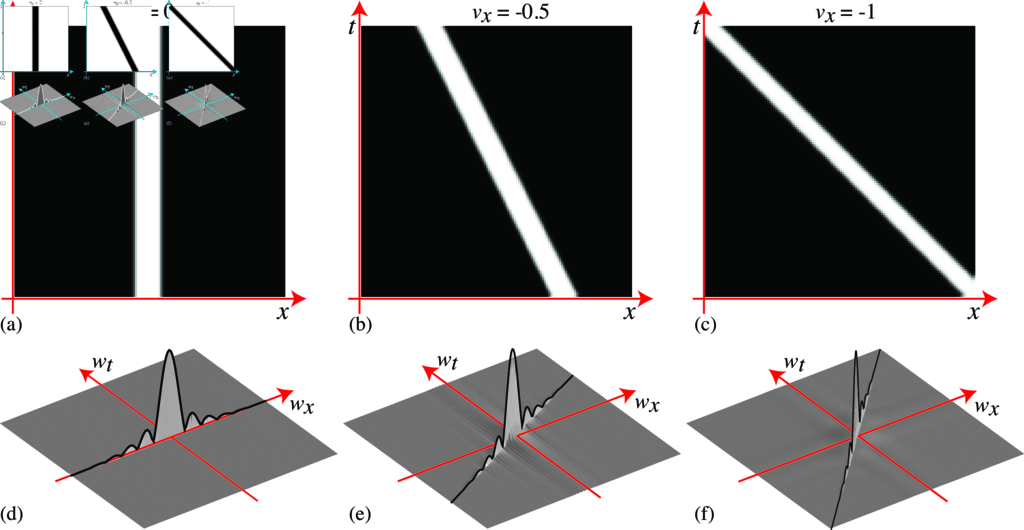
\includegraphics[width=1\linewidth]{figures/temporal_filters/mov_pulse_012.eps}
\caption{a) A sequence with one spatial dimension showing a static rectangular pulse. b) The rectangular pulse moves to the left at a speed $v=-0.5$ and c) moving towards the left, $v=-1$. As we work with discretized signals, speed units are in pixels per frame.} 
\label{fig:mov_pulse_012}
\end{figure}

Figure~\ref{fig:mov_pulse_012} shows the FT for a sequence with one spatial dimension, $f(x,t)$, that contains a blurry rectangular pulse moving at three different speeds towards the left. Fig.~\ref{fig:mov_pulse_012}.a shows a sequence when the pulse is static and fig.~\ref{fig:mov_pulse_012}.d shows its FT.  Across the spatial frequency $w_x$, the FT is approximately a sinc function. Across the temporal frequency $w_t$, as the signal is constant, its FT is a delta function.  Therefore the FT is a sinc function contained inside a delta wall in the line $w_t=0$. Fig.~\ref{fig:mov_pulse_012}.b shows the same rectangular pulse moving towards the left, $v_x=0.5$. Fig.~\ref{fig:mov_pulse_012}.e shows the sinc function but skewed a long the frequency line $w_t+0.5w_x=0$. Note that this is not a rotation of the sinc function from fig.~\ref{fig:mov_pulse_012}.d as the locations of the zeros lie at the same $w_x$ locations. Fig.~\ref{fig:mov_pulse_012}.c shows the pulse moving at a faster speed resulting in a larger skewing of its FT, Fig.~\ref{fig:mov_pulse_012}.f.


We let to the reader the work of computing its FT and visualizing the effect of the mask in the Fourier domain.



\section{Temporal filters}

Linear spatio-temporal filters can be written as spatio-temporal convolutions between the input sequence and a convolutional kernel (impulse response). Discrete spatiotemporal filters have an impulse response $h \left[n,m,t \right]$. The extension from 2D filter to spatio-temporal filters does not has any additional complications. We can also classify filters as low-pass, high-pass, etc. But in the case of time, there is another attribute used to characterize filters: causality. 
\begin{itemize} 
\item Causal filters: these are filters with output variations that only depend of the past values of the input. This puts the following constraint: $h \left[n,m,t \right]=0$ for all $t<0$. This means that if the input is an impulse at $t=0$, the output will only have non-zero values for $t>0$. If this condition is satisfied, then the filter output will only depend on the input's past for all possible inputs. 
\item Non-causal filters: when the output has dependency on future inputs.
\item Anti-causal filters: this is the opposite, when the output only depends on the future: $h \left[n,m,t \right]=0$ for all $t>0$.
\end{itemize}
Many filters are non-causal and have both causal and anti-causal components (e.g., a Gaussian filter). Note that non-causal filters can not be implemented in practice and, therefore, any filter with an anti-causal component will have to be approximated by a purely causal filter by bounding the temporal support and shifting in time the impulse response. 

In this chapter, we have written all the filters as convolutions. However, some filters are better described as difference equations (this is specially important in time). An example of a difference equation is:
\begin{equation}
g \left[n,m,t \right] = f \left[n,m,t \right] + \alpha \, h \left[n,m,t-1 \right]
\end{equation}
where the output $g$ at time $t$ depends on the input at time $t$ and the output at the previous time instant $t-1$ multiplied by a constant $\alpha$. We can easily evaluate the impulse response, $h \left[n,m,t \right]$, of such a filter by replacing $f\left[n,m,t \right]$ with an impulse, $\delta \left[n,m,t \right]$. The impulse response is:
\begin{equation}
h \left[n,m,t \right] = \alpha^t  \delta \left[n,m \right] u \left[t \right]
\end{equation}
where $u\left[t \right]$, called the Heaviside step function, is:
\begin{equation}
u \left[t \right] = \begin{cases}
    0     & \quad \text{if }  t <0 \\
    1     & \quad \text{otherwise }\\
\end{cases}
\end{equation}
Most filters described by differences equations have an impulse response with infinite support. They are called IIR (Infinite Impulse Response) filters. IIR filters can be further classified as stable and unstable. Stable filters are the ones that given a bounded input, $| f \left[n,m,t \right] |<A$, produce a bounded output, $| g \left[n,m,t \right] | <B$. For this to happen, the impulse response has to be bounded. In unstable filters, the amplitude of the impulse response diverges to infinity. In the previous example, the filter is stable if and only if $| \alpha | < 1$. 

Let's now describe some spatio-temporal filters. 


\subsection{Temporal Gaussian}

As with the spatial case, we can define the same low-pass filters: the box filter, triangular filters, etc.  As an example, let's focus on the Gaussian filter. The spatio-temporal gaussian is trivial extension of the spatial gaussian filter we have seen in section~\ref{sec:spt_gaussian}:
\begin{equation}
g(x,y,t; \sigma_x,\sigma_t) = \frac{1}{(2 \pi)^{3/2} \sigma_x^2\sigma_t} \exp{-\frac{x^2 +
   y^2}{2 \sigma_x^2}} \exp{-\frac{t^2}{2 \sigma_t^2}}
\label{eq:gauss3dcont}
\end{equation}
Where $\sigma_x$ is the width of the gaussian along the two spatial dimensions, and $\sigma_t$ is the width on the temporal domain. As the units for $t$ and $x,y$ are unrelated, it does not make sense to set all the $\sigma$s to have the same value. 

We can discretize the continuous gaussian by taking samples and building a 3D convolutional kernel. We can also use the binomial approximation. The 3D Gaussian is separable so it can be implemented efficiently as a convolutional cascade of 3 one dimensional kernels. Figure~\ref{fig:seq_filtered_kernel}.a shows a spatio-temporal gaussian. The temporal gaussian is a non-causal filter, therefore it is not physically realizable. This is not a problem when processing a video stored in memory. However, if we are processing an streamed video, we will have to bound and shift the filter to make it causal which will result in a delay in the output. 

Figure~\ref{fig:sec_filtered_blur}.a shows one sequence and figure~\ref{fig:sec_filtered_blur}.b shows the sequence filtered with the gaussian from figure~\ref{fig:seq_filtered_kernel}.a.This Gaussian has a small spatial width, $\sigma=1$, and a large temporal width, $\sigma_t=4$ so the sequence is strongly blurred across time. The moving objects show motion blur and are strongly affected by the temporal blur, while the static background is only affected by the spatial width of the gaussian.

\begin{figure}
\includegraphics[width=1\linewidth]{figures/temporal_filters/seq_filtered_kernel.eps}
\caption{a) Spatio-temporal Gaussian with $\sigma=1$ and $\sigma_t=4$.  b) Same gaussian parameters but skewed by the velocity vector $v_x=-1, v_y=0$ pixels/frame, c) and $v_x=1, v_y=0$ pixel/frame.} 
\label{fig:seq_filtered_kernel}
\end{figure}

How could we create a filter that keeps sharp objects that move at some velocity $(v_x,v_y)$ while blurring the rest? Figure~\ref{fig:sec_filtered_blur}.c shows the desired output of such a filter. The bottom image shows one frame for a sequence filtered with a kernel that keeps sharp objects moving left at 1 pixel/frame while blurring the rest. This filter can be obtained by skewing the gaussian:
\begin{equation}
g_{v_x,v_y}(x,y,t) = g(x - v_xt,y - v_yt, t) 
\end{equation}
%where $g_{v_x,v_y}(x,y,t)$ is a skewed gaussian a long the space-time direction $(v_x,v_y,1)$. 
This directional blur is not a rotation of the original Gaussian as the change of variables is not unitary, but the same effect could be obtained with a rotation. Figure~\ref{fig:sec_filtered_blur}.c shows the effect when $v_x=-1, v_y=0$. The gaussian is shown in fig.~\ref{fig:seq_filtered_kernel}.b. The space-time section shows how the sequence is blurred everywhere except one oriented bad corresponding to the person walking left. Figure~\ref{fig:sec_filtered_blur}.d shows the effect when $v_x=1, v_y=0$. The output of this filter looks as if the camera was tracking one of the objects while the shutter was open, producing a blurry image of all the other objects.

\begin{figure}
\includegraphics[width=1\linewidth]{figures/temporal_filters/seq_filtered_blur.eps}
\caption{a) One frame from the input sequence and the space-time section (on top). b) Output when convolving the the gaussian from fig.~\ref{fig:seq_filtered_kernel}.a. c) Output of the convolution with fig.~\ref{fig:seq_filtered_kernel}.b, and d) output of the convolution with fig.~\ref{fig:seq_filtered_kernel}.c.} 
\label{fig:sec_filtered_blur}
\end{figure}


\subsection{Temporal derivatives}

Spatial derivatives were useful to find regions of image variation such as object boundaries. Temporal derivatives can be used to locate moving objects. We can approximate a temporal derivative for discrete signals as:
\begin{equation}
f \left[m,n,t\right] - f \left[m,n,t-1\right] 
\end{equation}

As in the spatial case, it is useful to compute temporal derivatives of spatio-temporal gaussians:
\begin{equation}
\frac{\partial g}{\partial t} = \frac{-t}{\sigma_t^2} g(x,y,t)
\end{equation}
where $g(x,y,t)$ is the Gaussian as written in eq.~\ref{eq:gauss3dcont}. We can compute the spatio-temporal gradient of a gaussian:
\begin{equation}
\nabla  g = \left( g_x(x,y,t), g_y(x,y,t), g_t(x,y,t) \right) =  \left(-x/\sigma^2, -y/\sigma^2, -t/\sigma_t^2 \right) g(x,y,t)
\end{equation}


What should we do if we want to remove only the objects moving at a particular velocity? 

In the case of a moving image with velocity $(v_x, v_y)$, the sequence is $f (x,y,t) = f_0 (x-v_xt,y-v_yt)$, we can compute the temporal derivative of $f(x,y,t)$ as:
\begin{equation}
\frac{\partial f}{\partial t} = \frac{\partial f_0}{\partial t} = -v_x \frac{\partial f_0}{\partial x} - v_y \frac{\partial f_0}{\partial y}
\label{eq:brightnessconstancy}
\end{equation}

\begin{figure}
\includegraphics[width=1\linewidth]{figures/temporal_filters/gaussians_xyt_seq.eps}
\caption{Visualization of the space-time Gaussian. The gaussian has a width of $\sigma^2=\sigma_t^2=1.5$, and has been discretized as a 3D array of size $7 \times 7 \times 7$. Each image shows one frame. a)  Gaussian b) The partial derivative of the Gaussian with respect to $t$. c) Derivative along $v=(1,0)$ pixels/frame. d) $v=(-1,0)$ pixels/frame.} 
\label{fig:gaussian_seq}
\end{figure}

\begin{figure}
\includegraphics[width=1\linewidth]{figures/temporal_filters/gaussians_xyt_section.eps}
\caption{Spatio-temporal Gaussian $g\left[ n,t \right]$ and derivatives. a) Gaussian with $\sigma^2=1.5$. b) Partial derivative with respect to $t$. c) Partial derivative along $(1,-1)$, d) Partial derivative along $(1,1)$.} 
\label{fig:gaussian_xyt_section}
\end{figure}

If we compute the gradient of the gaussian along the vector $\left[1,v_x,v_y\right]$:
\begin{equation}
h(x,y,t;v_x,v_y) = g_t+v_xg_x+v_yg_y = \nabla  g \left( 1,v_x,v_y \right)^T
\end{equation}
and we convolve it with $f_0 (x-v_xt,y-v_yt)$ we get a zero output (using eq.~\ref{eq:brightnessconstancy}):
\begin{eqnarray}
f_0 (x-v_xt,y-v_yt) \circ h &=& f_0 (x-v_xt,y-v_yt) \circ \left(  g_t+v_xg_x+v_yg_y \right) \\
&=& \left( \frac{\partial f_0}{\partial t} + v_x \frac{\partial f_0}{\partial x} + v_y \frac{\partial f_0}{\partial y} \right) \circ g \\
&=& 0
\end{eqnarray}
The filter $h$ is shown in figure \ref{fig:gaussian_seq} as a sequence for different velocities. In the example shown in the figure, the gaussian (fig.~\ref{fig:gaussian_seq}.a) has a width of $\sigma^2=\sigma_t^2=1.5$, and has been discretized as a 3D array of size $7 \times 7 \times 7$. Figures b,c and d  show the filter $h$ for different velocities: $(v_x,v_y) =$ $(0,0)$, $(1,0)$ and $(-1,0)$. Fig.~\ref{fig:gaussian_xyt_section} shows the corresponding space-time sections of the same spatio-temporal gaussian derivatives. Both visualizations are equivalent and help to understand how the filter works.
%
%This is because we are computing spatio-temporal derivatives a long the direction of motion, so any object moving at that particular speed will be a constant a long that direction and its derivative will be zero. Fig.~\ref{fig:gaussian_xyt_section} shows a discrete spatio-temporal gaussian and temporal derivatives. Fig.~\ref{fig:gaussian_xyt_section}.a shows the gaussian across one spatial dimension and time. Fig.~\ref{fig:gaussian_xyt_section}.b is the temporal derivative, Fig.~\ref{fig:gaussian_xyt_section}.c shows the discretized gaussian gradient $g_t \left[n,t \right]+v_x g_x \left[ n,t \right]$ with $v_x=-1$ and Fig.~\ref{fig:gaussian_xyt_section}.d with $v_x=1$.


Such a filter will cancel any objects moving at the velocity $(v_x,v_y)$. By using different filters, each one computing derivatives a long different space-time orientations, we 



\begin{figure}
\includegraphics[width=1\linewidth]{figures/temporal_filters/seq_filtered_der.eps}
\caption{a) Input sequence. b) $v_x=v_y=0$, c) $v_x=1$ pixels/frame. d) $v_x=-1$ pixel/frame.} 
\label{fig:tunedfilter}
\end{figure}


%\subsubsection{Motion detectors}
%
%Reighart model of the fly visual system?
%
%Maybe this is better later because it uses a battery of filters.


%FIGURE: velocity tunning? Compute the energy of the output as a function of the input velocity. This shows that fr large velocities the tunning is not tight. 



\subsection{Spatiotemporal Gabor filters}

\begin{figure}
\centerline{
\includegraphics[width=1\linewidth]{figures/temporal_filters/gabor_spacetime_FT.eps}
}
\caption{Space-time Gabor filters. a) Cosine and sine $x$-$t$ Gabor filter, and b) the sketch of its transfer function. c) Sketch of the transfer function of a spatiotemporal Gabor filter in 2 spatial dimensions ($x$-$y$-$t$).}
\label{fig:spacetimefilts}
\end{figure}


Just as we did with Gaussian derivatives, extending Gabor filter for motion analysis is a direct generalization of the x-y 2D Gabor function to a x-y-t 3D Gabor function. Figure~\ref{fig:spacetimefilts}.a shows a x-t (cosine and sine) Gabor function in 1 spatial dimension, and  Figure~\ref{fig:spacetimefilts}.b shows a sketch of its Fourier transform. This function is selective to signals translating to the right with a speed $v=1$, i.e. $f(x-t)$. The red line in Figure~\ref{fig:spacetimefilts}.b shows Dirac line that contains the energy of the moving signal. 

In 2 spatial dimensions, Figure~\ref{fig:spacetimefilts}.c shows the sketch of the Gabor transfer function. Note that the x-y-t Gabor filter is not selective to velocity. If we have a 2D moving signal $f(x-v_xt, y-v_yt)$, the Fourier transform is contained inside a Dirac plane. Therefore, there are an infinite number of planes that will pass by the frequencies of the Gabor filter. All those planes intersect the red line shown in Figure~\ref{fig:spacetimefilts}.c. A single Gabor filter can not disambiguate the input velocity. 

Equation of the velocity as a function of the frequency tuning.


\section{Velocity-tuned filters}
\label{sect:velocityTunedFilters}

How can we measure input velocity? There are many different approaches in the computer vision community
for measuring motion.  Here we show that it is possible
to measure motion even with the simple processing machinery that
we've developed so far.

\begin{figure}
\centerline{
\includegraphics[width=1\linewidth]{figures/temporal_filters/gabor_spacetime_tiles.eps}
}
\caption{a) Space-time Gabor filters tiles. b) Set of Gabor filters selective to a particular velocity.}
\label{fig:spacetimetiles}
\end{figure}



We can use quadrature pairs of oriented filters in space-time to find motion
speed and direction in the video signal.  We just need to find the
space-time orientation of strongest response. Figure \ref{fig:spacetimefilts}.a shows a set of Gabor filters sampling the space-time frequency domain. When the input contains a moving signal, we can use a set of filters to identify the plane in the Fourier domain that contains the input energy. Figure \ref{fig:spacetimefilts}.b shows the subset of filters that have the strongest output for a particular input motion. 


As an illustration, Figure~\ref{fig:MT_velocity_tuned} shows one possible architecture to create velocity-selective units. The first layer is composed by Gabor filters (cosine and sine) which are frequency-selective units. The outputs are combined according to different planes in the Fourier domain to create velocity-selective outputs. 

Given an input sequence, one can estimate velocity by looking at the velocity-tuned unit with the strongest response. 

\begin{figure}
\centerline{
\includegraphics[width=1\linewidth]{figures/temporal_filters/MT_velocity_tuned.eps}
}
\caption{Architecture to create velocity-selective units. The first layer is composed by space-time Gabor filters (cosine and sine) which are frequency-selective units. Here we represent the impulse response of each filter by a small x-y-t cube. For each quadrature pair we compute the amplitude. Then amplitude outputs are combined according to form different planes in the Fourier domain to create velocity-selective outputs. A normalization layer can be added to normalize the outputs by dividing every output by the sum of all the amplitudes (not shown). The full architecture is non-linear.}
\label{fig:MT_velocity_tuned}
\end{figure}

\section{Human Motion Processing}
\reviewcomment{Figures need reformatting.}

While researchers aren't sure of the precise computations involved in human motion processing, some experiments  can distinguish between classes of algorithms that the visual system may use.  The methods of the previous section are based on {\em spatio-temporal filtering} \cite{Adelson85}.  A second class of motion algorithms includes correlation-based methods, and can be called {\em pattern matching methods} \cite{Adelson85}.  In such methods, the motion offset of a spatial pattern from some starting position is computed by finding the position of highest correlation with the spatial pattern.

Adelson and Bergen proposed a beautiful motion illusion that distinguishes between two classes of motion algorithms that might be used by the visual system.  The illusion involves temporal filtering, motion processing, and aliasing and so provides a good review of the material in this chapter.

The illusion is presented in the video in Fig.~\ref{fig:blends}. The signals, and magnitudes of their space-time Fourier transforms, are developed in Figs.~\ref{fig:motionIllusion1} and \ref{fig:motionIllusion2}, building-up from simpler signals.  The three rows of Fig.~\ref{fig:motionIllusion1} show a stationary sinusoid, a moving sinusoid, and a moving square-wave.  The spatio-temporal Fourier transform of the stationary sinusoid, $I(x) = \cos(\pi \omega x)$ is $\delta(\nu) (\delta(\omega) + \delta(-\omega))$.  We have added a constant bias to the sinusoid to avoid negative intensity values, leading to an impulse at the center of the Fourier transform figure, Fig.~\ref{fig:motionIllusion1}~(c).  The resulting 3 colinear impulses are along the temporal frequency, $\nu = 0$ line.  A space-time plot of the signal, Fig.~\ref{fig:motionIllusion1}~(b), shows only vertical structures, indicating no motion.

A moving sinusoid has a similar Fourier transform magnitude, Fig.~\ref{fig:motionIllusion1}~(f), but with the spatio-temporal energies along a line perpendicular to the moving structures in the spatio-temporal signal, Fig.~\ref{fig:motionIllusion1}~(e).  A moving square wave is similar, but the extra harmonics needed to construct the square wave visible in the Fourier transform, Fig.~\ref{fig:motionIllusion1}~(i).

Continuing the development of the illusion, Fig.~\ref{fig:motionIllusion2}~(c) shows the Fourier transform and space-time plot of a square-wave moving in 1/4 period jumps each time increment.  This signal can be formed from Fig.~\ref{fig:motionIllusion1}~(h) by applying a periodic sample-and-hold function, resulting in the spectrum of  Fig.~\ref{fig:motionIllusion1}~(i) replicated over temporal frequencies, and multiplied by a sinc function over temporal frequency.  The resulting Fourier transform magnitude is shown in Fig.~\ref{fig:motionIllusion2}~(c).  

Because orientation in space-time tells motion direction, Sect.~\ref{sect:modelingSequences}, the space-time plot of Fig.~\ref{fig:motionIllusion2}~(b) shows that the motion should be perceived to left.  This will be consistent with the behavior of velocity tuned filters, Sect.~\ref{sect:velocityTunedFilters}, responding to the lowest spatio-temporal frequency impulses shown in 
Fig.~\ref{fig:motionIllusion2}~(c). However, if we remove the lowest spatial frequency sinusoid from the signal, the result is shown in 
Fig.~\ref{fig:motionIllusion2}~(e), with spatio-temporal Fourier transform Fig.~\ref{fig:motionIllusion2}~(g).  Now the lowest spatio-temporal frequency cosine wave is oriented in the other direction.  This opposite slope is also visible in the spatial domain, in the space-time plot of Fig.~\ref{fig:motionIllusion2}~(e), and especially if we low-pass filter that, resulting in Fig.~\ref{fig:motionIllusion2}~(f).

The signal of the second row of Fig.~\ref{fig:motionIllusion2} poses a conundrum.  It can be argued that the signal moves to the left, just as does the signal of row 1 of Fig.~\ref{fig:motionIllusion2}.  The pattern match--the minimum correlation signal--indeeds move to the left.  But vision system examining the orientation of the lowest spatio-temporal frequency components of the signal in Fig.~\ref{fig:motionIllusion2}~(g), or looking at the dominant orientations in the space-time plots of 
 Fig.~\ref{fig:motionIllusion2}~(e) and (g), would find a signal moving to the right.
 
 How does the signal appear to move to you?  We invite you to play the videos of Fig.~\ref{fig:motionIllusion2}~(c) and (g) (set your player to loop the videos) to assess which way each of the signals of  Fig.~\ref{fig:motionIllusion2} moves.   Fig.~\ref{fig:blends} show slow and fast motion versions of a blended signal, where the top half contains the lowest sinusoidal spatial frequency component of the square wave and the bottom half does not.  By moving your eye vertically, you can convince yourself that the entire pattern is moving rigidly to the left, yet it also appears that the top half is moving to the left and the bottom half is moving to the right.  This demonstration gives evidence for spatio-temporal filter-based motion processing within the human visual system, since such filtering would predict leftward motion for the top halves of the videos in Fig.~\ref{fig:blends}, and rightward motion for the bottom halves of those videos.

\begin{figure}
\centerline{
\hspace{-0.2in}
\sublabelnp{(a) 
\href{https://groups.csail.mit.edu/vision/cvbook/videos/stillsineLoop.mov}{stationary sine wave (click for video)}}
{
\href{https://groups.csail.mit.edu/vision/cvbook/videos/stillsineLoop.mov}{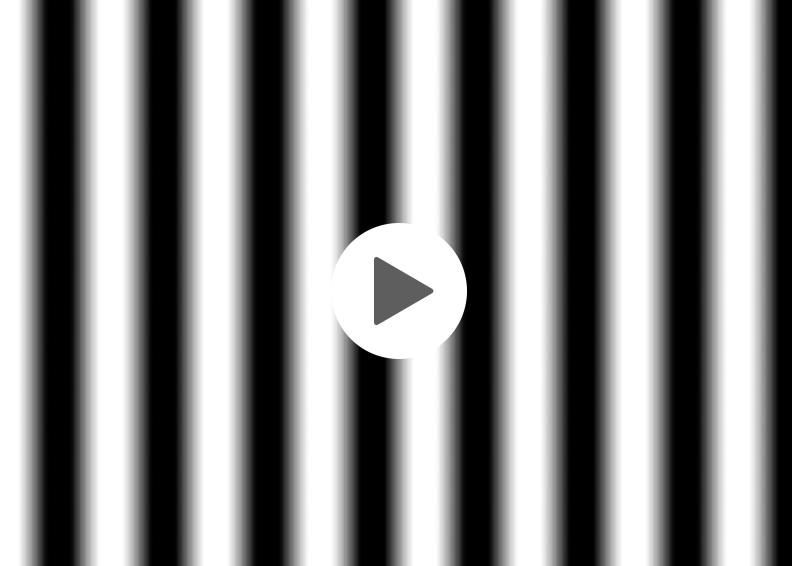
\includegraphics[width=0.2\linewidth]{figures/temporal_filters/movie1.jpg}}}
\sublabelnp{(b) space-time image}{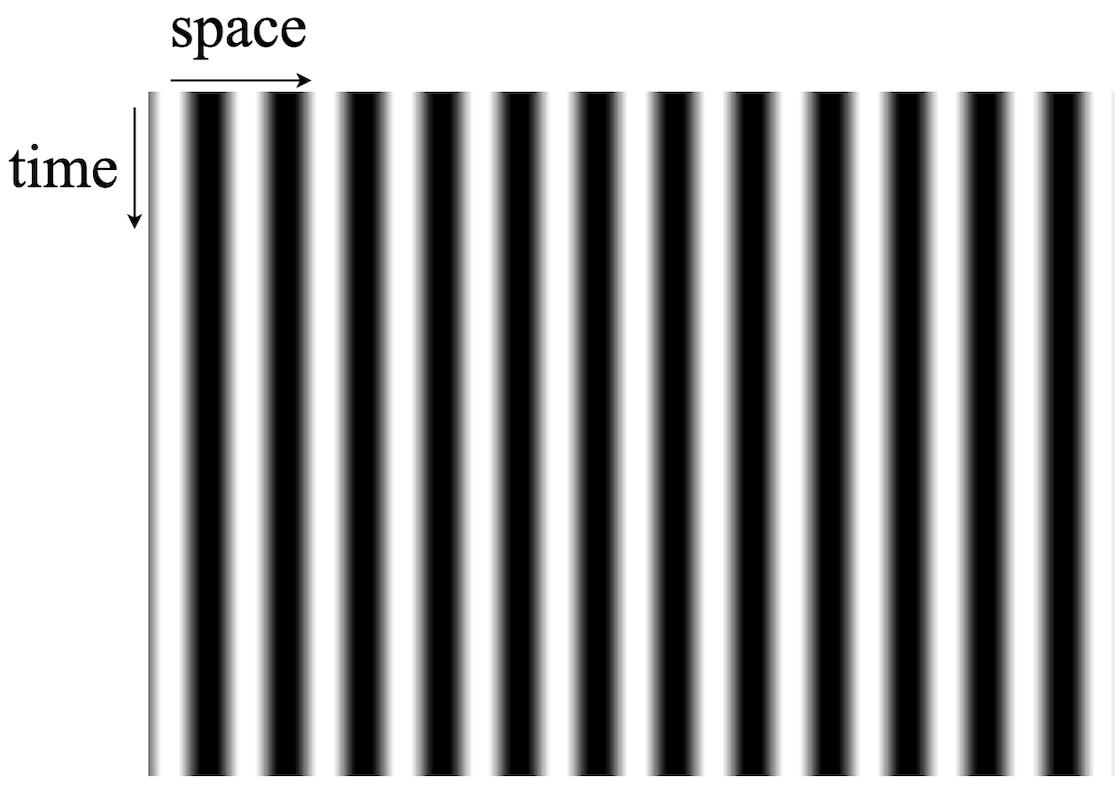
\includegraphics[width=0.3\linewidth]{figures/temporal_filters/st1a.jpg}}
\sublabelnp{(c) space-time Fourier transform}{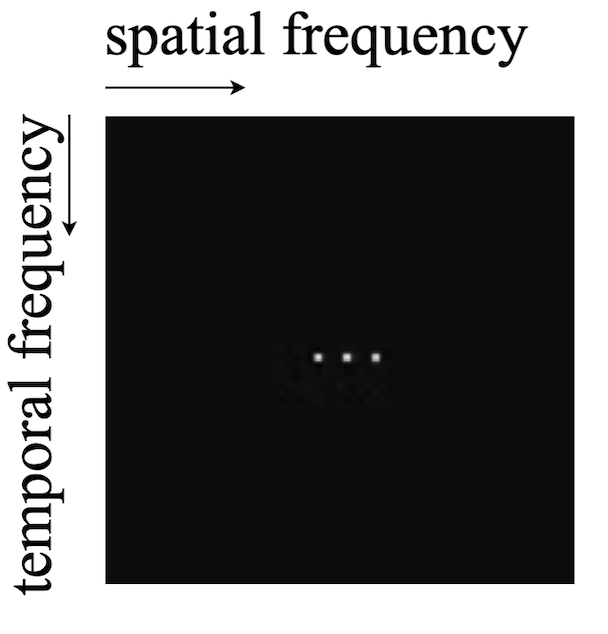
\includegraphics[width=0.3\linewidth]{figures/temporal_filters/stdft1.jpg}}}
\centerline{
\sublabelnp{(d) 
\href{https://groups.csail.mit.edu/vision/cvbook/videos/movingSineLoop.mov}{moving sine wave (click for video)}
}
{
\href{https://groups.csail.mit.edu/vision/cvbook/videos/movingSineLoop.mov}{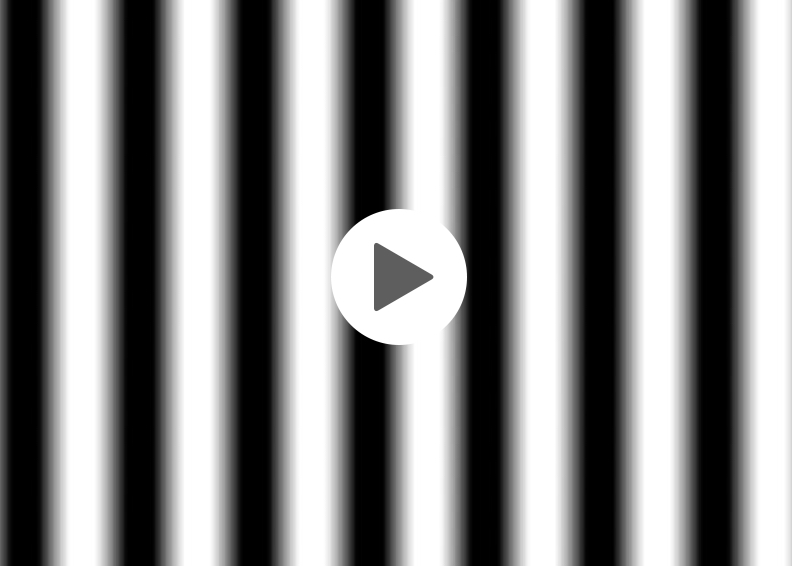
\includegraphics[width=0.2\linewidth]{figures/temporal_filters/movie2.jpg}}}
\hspace{0.1in}
\sublabelnp{(e) space-time image}{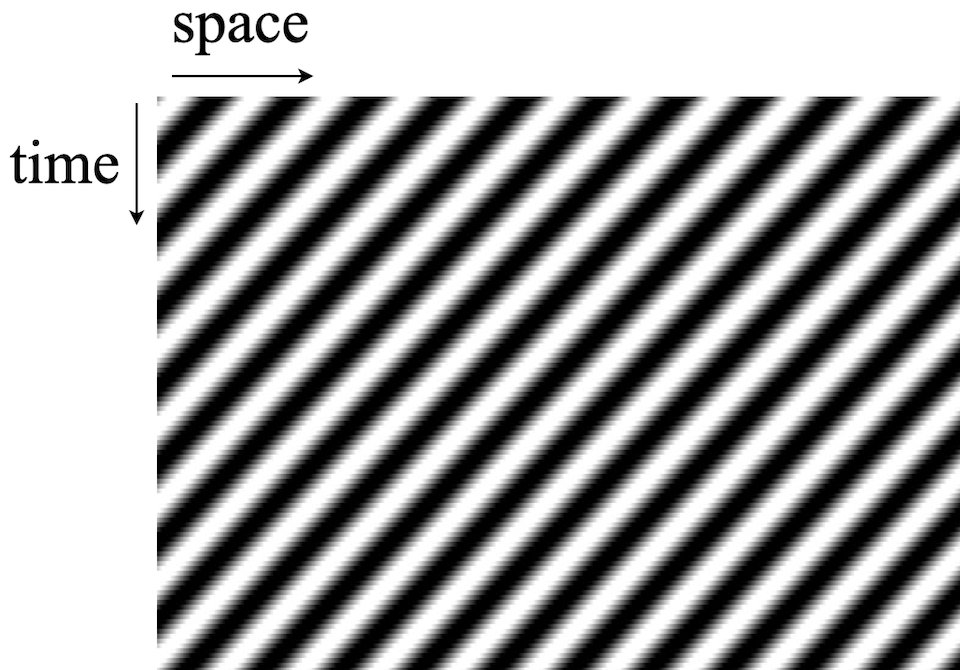
\includegraphics[width=0.3\linewidth]{figures/temporal_filters/st2.jpg}}
\hspace{0.5}
\sublabelnp{(f) space-time Fourier transform}{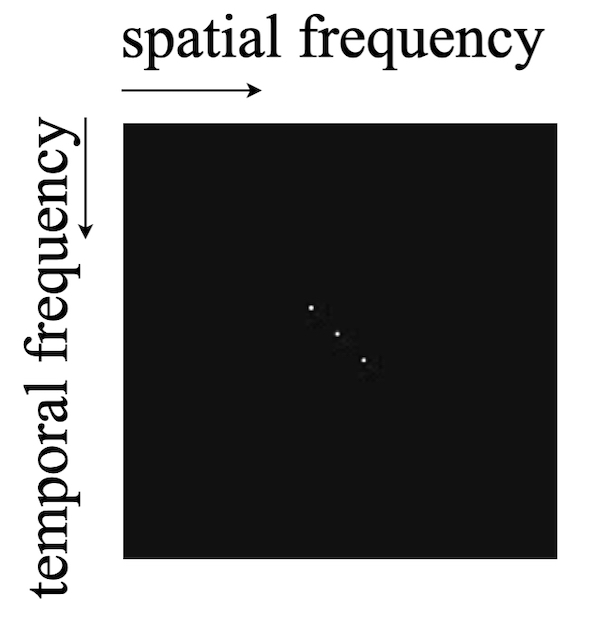
\includegraphics[width=0.3\linewidth]{figures/temporal_filters/stdft2.jpg}}
}
\centerline{
\sublabelnp{(g) 
\href{https://groups.csail.mit.edu/vision/cvbook/videos/movingSquareLoop.mov}{moving square wave (click for video)}
}
{
\href{https://groups.csail.mit.edu/vision/cvbook/videos/movingSquareLoop.mov}{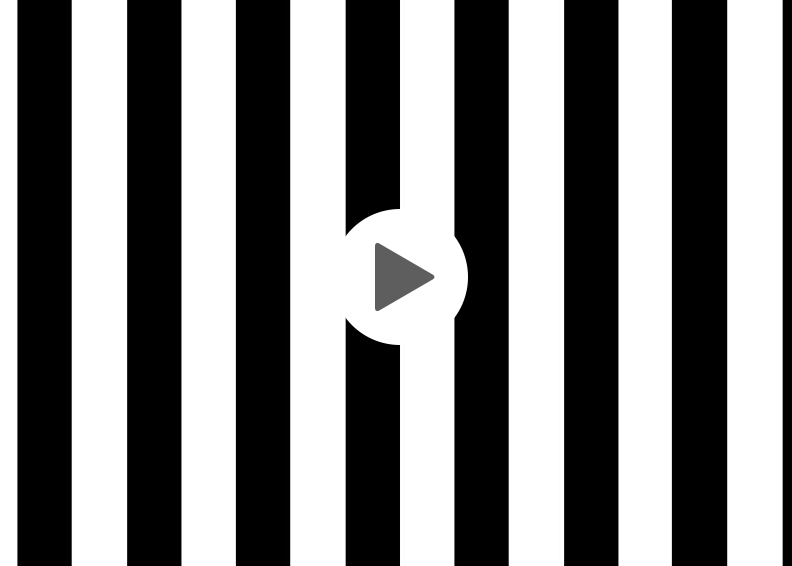
\includegraphics[width=0.2\linewidth]{figures/temporal_filters/movie3.jpg}}}
\hspace{-0.8}
\sublabelnp{(h) space-time Fourier transform}{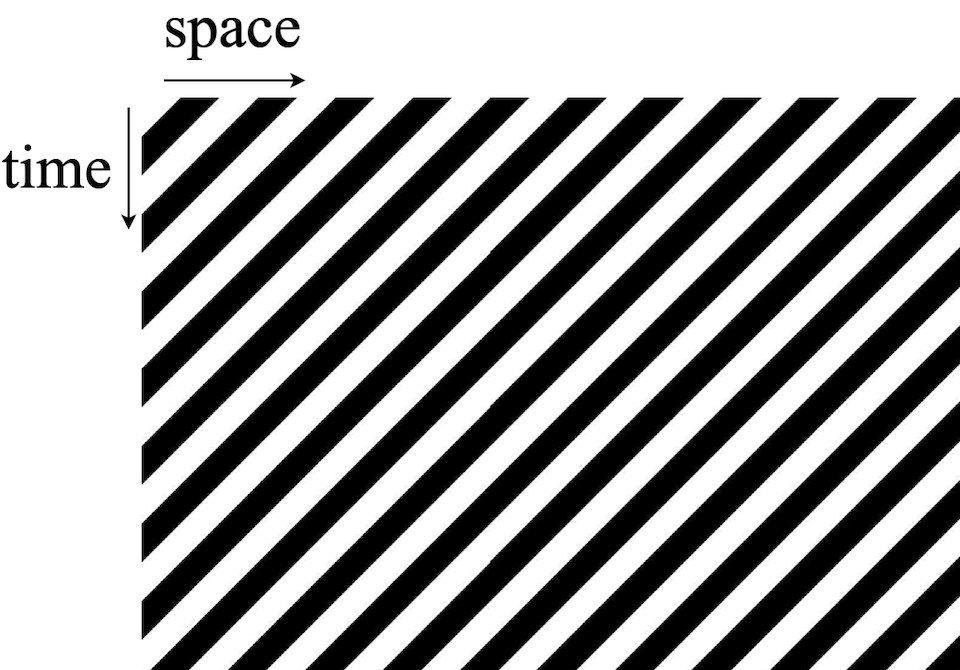
\includegraphics[width=0.3\linewidth]{figures/temporal_filters/st3.jpg}}
\hspace{-0.1in}
\sublabelnp{(i) space-time Fourier transform}{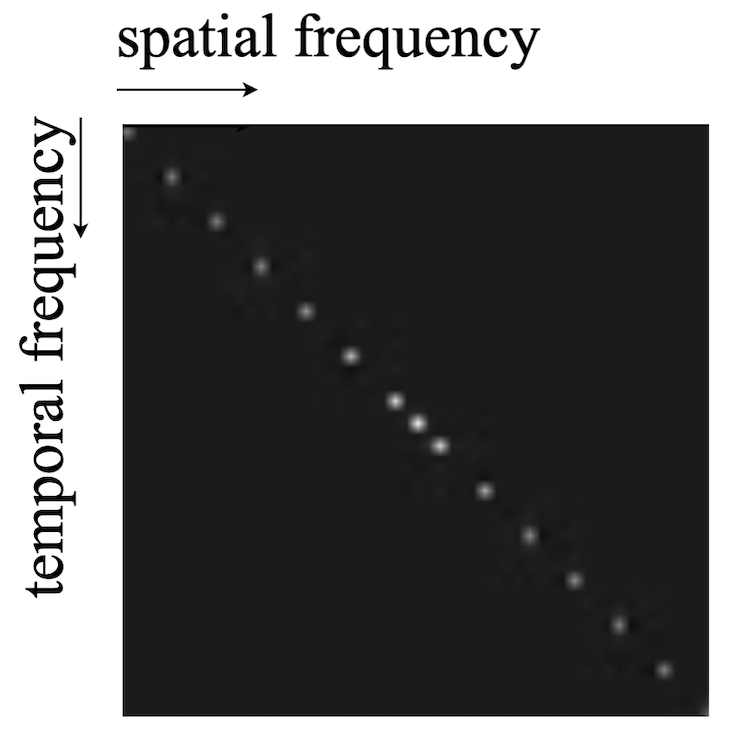
\includegraphics[width=0.3\linewidth]{figures/temporal_filters/stdft3.jpg}}
}
\caption{Space-time signals, building toward the fluted square-wave motion illusion.    First row: stationary sine wave, (a) Movie of a motionless sine wave. (b) The space-time plot shows only vertical structure. 
(c) spatio-temporal Fourier transform has all energy on the zero temporal frequency axis, since nothing is moving.
Second row:  (d) moving sine wave. (e) In the space-time plot, speed corresponds to local orientation. (f) The Fourier transform energy is sheared according to the sine wave's speed.   
Third row:  Moving square wave.  The additional harmonics required to form a square wave are visible in the spatio-temporal Fourier transform, (i).  }
\label{fig:motionIllusion1}
\end{figure}

\begin{figure}
\centerline{
\sublabelnp{(a) 
\href{https://groups.csail.mit.edu/vision/cvbook/videos/steppedSquareLoop.mov}{stepped square wave (click for video)}
}
{
\href{https://groups.csail.mit.edu/vision/cvbook/videos/steppedSquareLoop.mov}{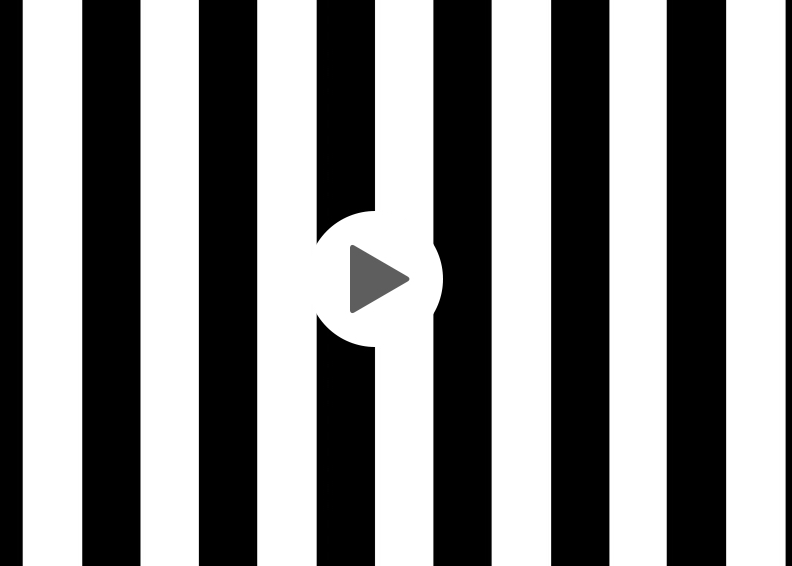
\includegraphics[width=0.2\linewidth]{figures/temporal_filters/movie4.jpg}}}
\sublabelnp{(b) space-time image}{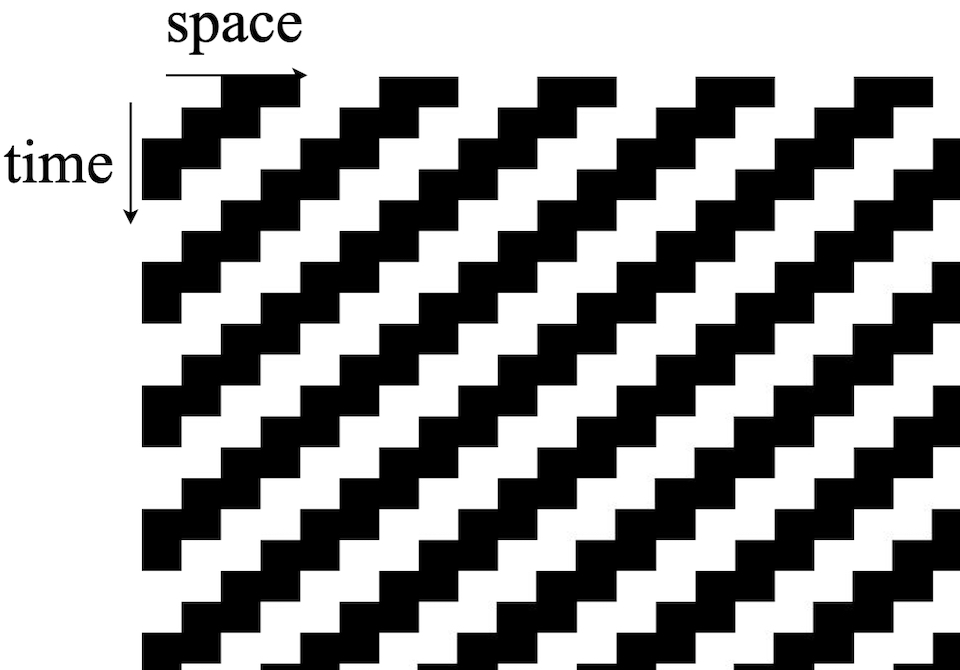
\includegraphics[width=0.3\linewidth]{figures/temporal_filters/st4.jpg}}
\sublabelnp{(c) space-time Fourier transform}{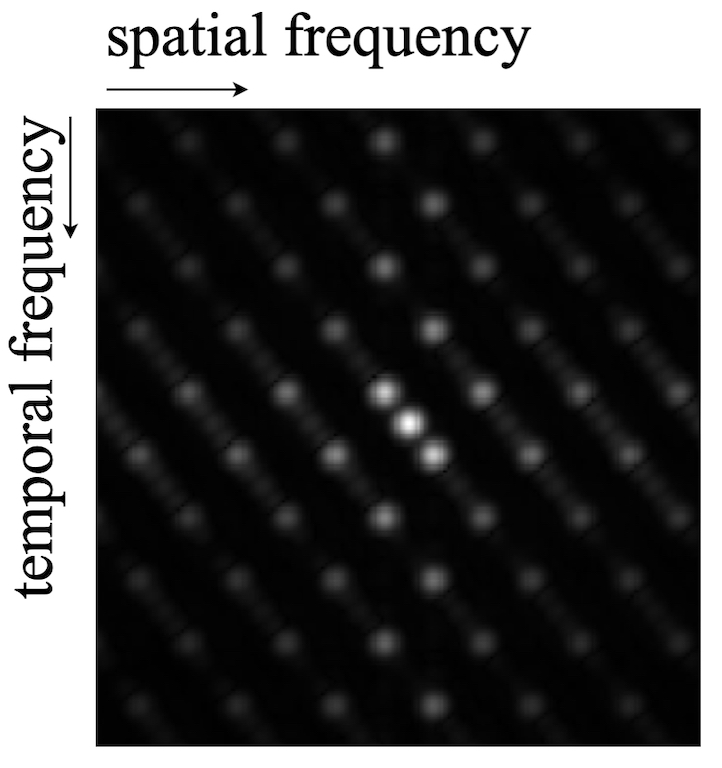
\includegraphics[width=0.3\linewidth]{figures/temporal_filters/stdft4.jpg}}
}
\centerline{
\hspace{-0.6in}
\sublabelnp{(d) 
\href{https://groups.csail.mit.edu/vision/cvbook/videos/steppedFlutedSquareLoop.mov}{fluted square wave  (click for video)}
}
{
\href{https://groups.csail.mit.edu/vision/cvbook/videos/steppedFlutedSquareLoop.mov}{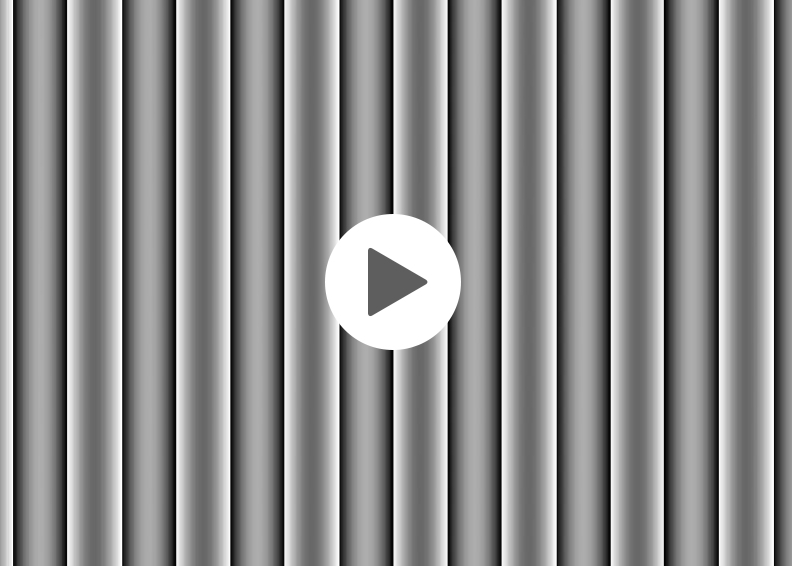
\includegraphics[width=0.2\linewidth]{figures/temporal_filters/movie5.jpg}}}
\hspace{-0.6in}
\sublabelnp{(e) space-time image}{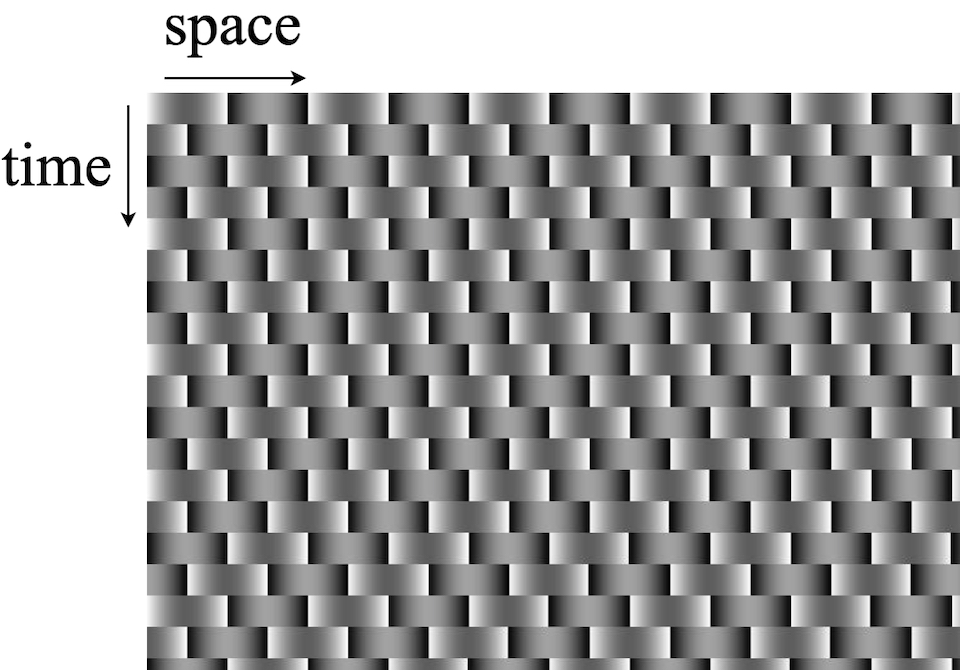
\includegraphics[width=0.27\linewidth]{figures/temporal_filters/st5.jpg}}
\hspace{-0.2in}
\sublabelnp{(f) space-time Fourier transform}{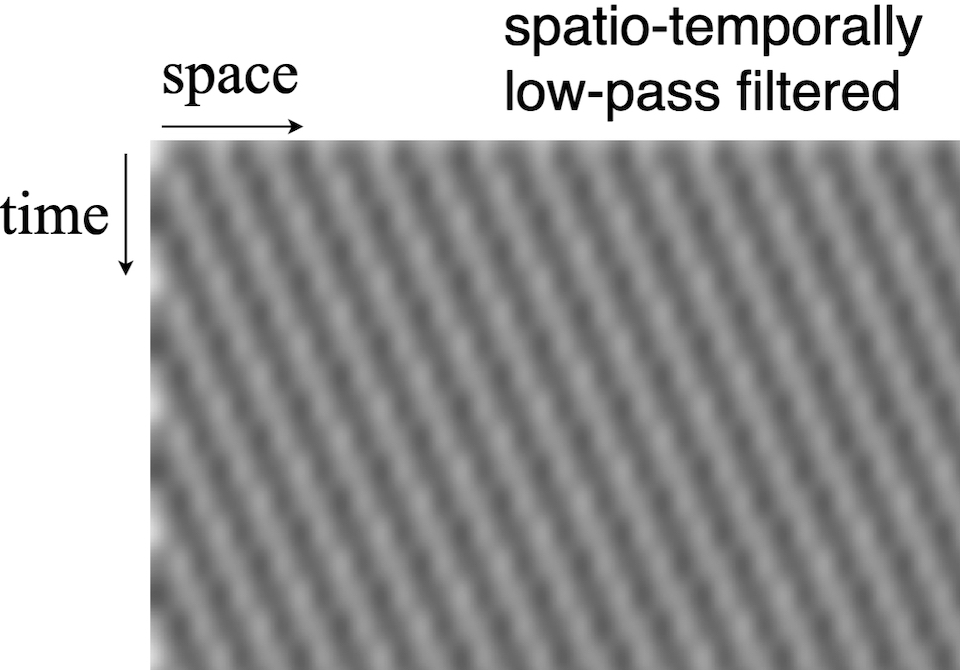
\includegraphics[width=0.3\linewidth]{figures/temporal_filters/st6.jpg}}
\hspace{-0.4in}
\sublabelnp{(g) space-time Fourier transform}{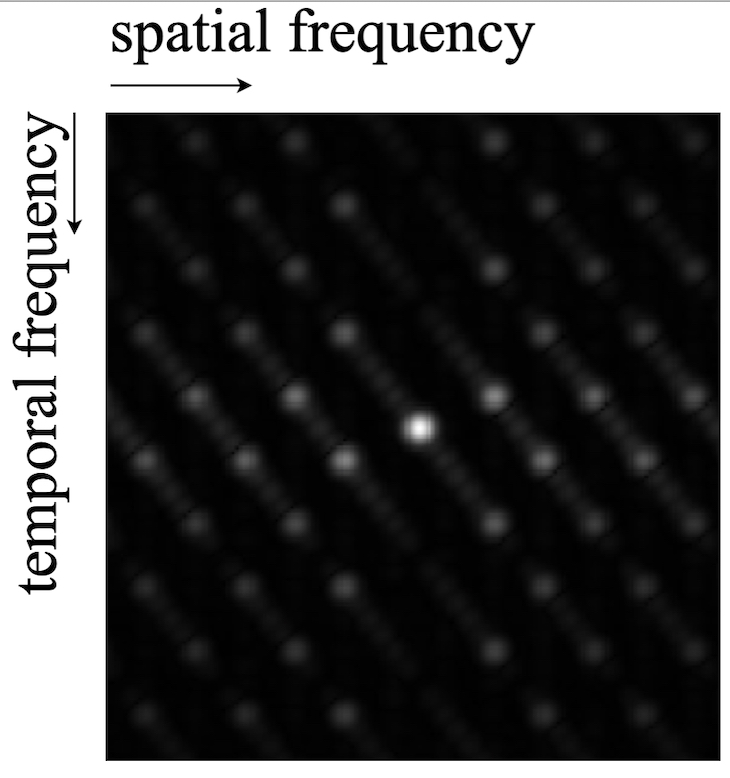
\includegraphics[width=0.3\linewidth]{figures/temporal_filters/stdft5.jpg}}
}
\caption{Derivation of the fluted square-wave motion illusion, continued from Fig.~\ref{fig:motionIllusion1}.  First row:  This square wave moves in 1/4 wavelength jumps, instead of continuously.  This staggered motion generates the additional spatio-temporal frequencies shown in (a).  The lowest spatio-temporal frequency still indicates motion to the left.  Second row:  If we remove the lowest spatial frequency sine wave of the square wave, creating a "fluted square wave", then the lowest spatio-temporal frequency now moves in the other direction.  This is also visible from the space time plot in (e), and especially in the spatio-temporally low-pass filtered version, (f).}
\label{fig:motionIllusion2}
\end{figure}



\begin{figure}
\centerline{
\sublabelnp{(a) 
\href{https://groups.csail.mit.edu/vision/cvbook/videos/blendedSlowLoop.mov}{motion illusion, slow (click for video)}
}
{
\href{https://groups.csail.mit.edu/vision/cvbook/videos/blendedSlowLoop.mov}{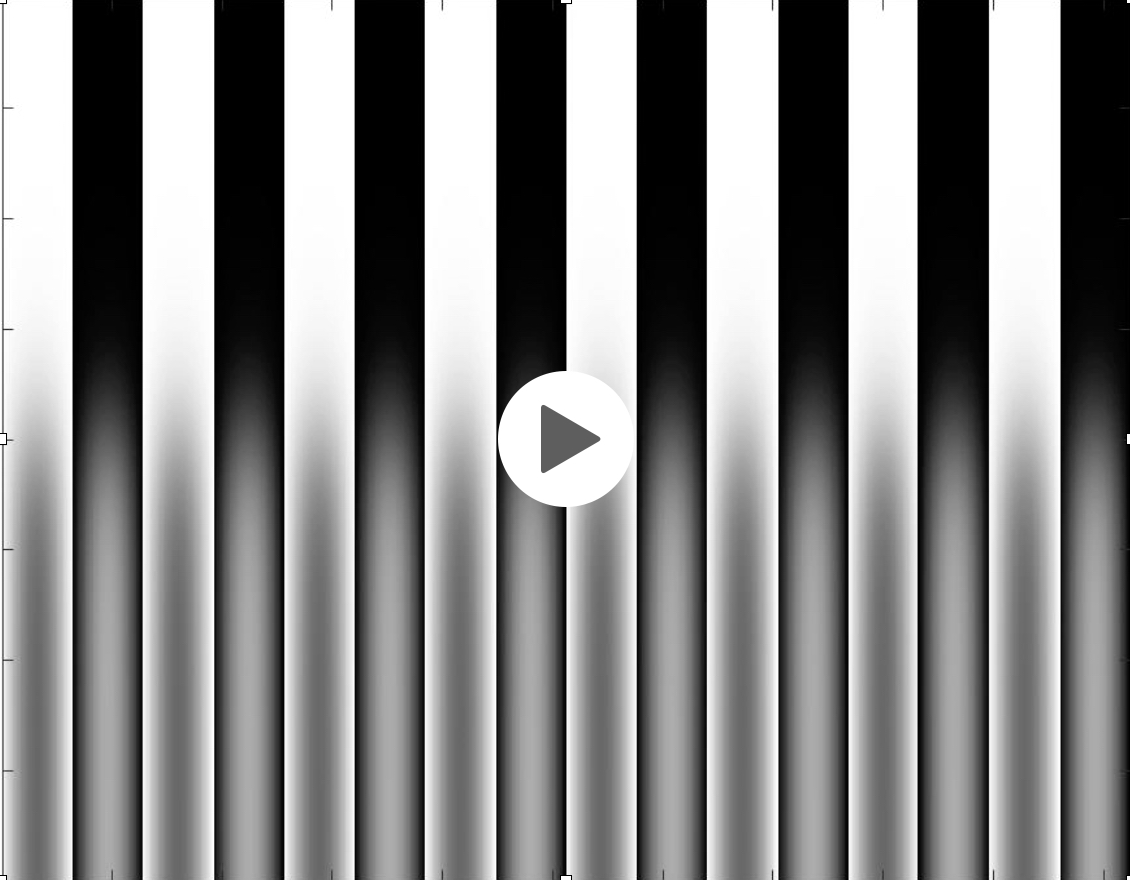
\includegraphics[width=0.2\linewidth]{figures/temporal_filters/blendFrame.jpg}}}
\sublabelnp{(b) 
\href{https://groups.csail.mit.edu/vision/cvbook/videos/fastBlendLoop.mov}{motion illusion, fast (click for video)}
}
{
\href{https://groups.csail.mit.edu/vision/cvbook/videos/fastBlendLoop.mov}{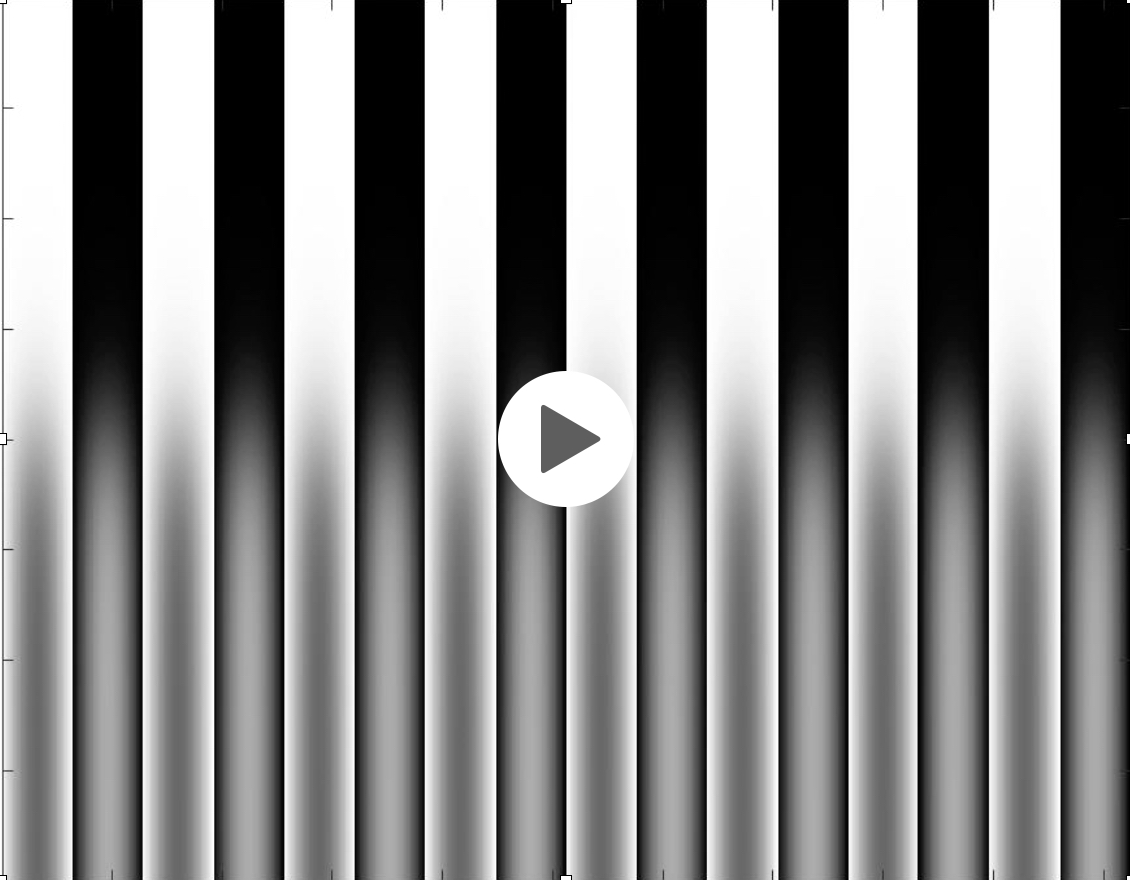
\includegraphics[width=0.2\linewidth]{figures/temporal_filters/blendFrame.jpg}}}
}
\caption{"Impossible combination" of ordinary and  fluted square-waves (view on looping display).  While one can verify, by tracing a finger or scanning your eyes, that the entire structure is moving rigidly to the left, the bottom half appears to be moving to the right.  At a fast speed, (b), the effect is accentuated.}
\label{fig:blends}
\end{figure}



%Here's a mock-up of a real scene.  We have a stationary background,
%and two cars driving in opposite directions.  (Thanks to Anat Levin
%for creating this slide).
%
%
%\begin{figure}
%\centerline{
%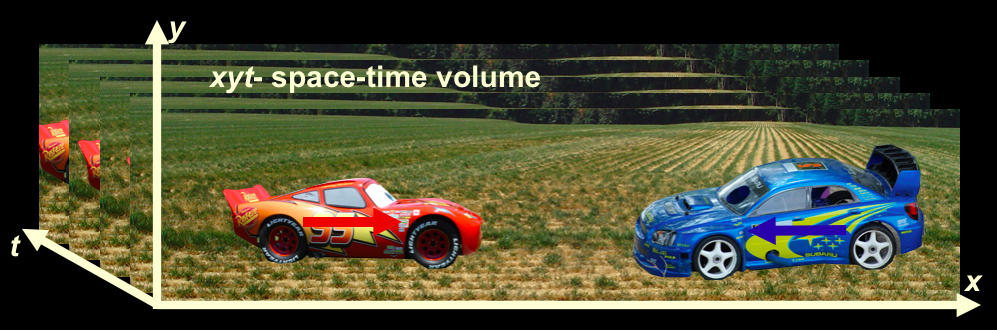
\includegraphics[width=0.6\linewidth]{figures/figs3/cars1.jpg}
%}
%\centerline{
%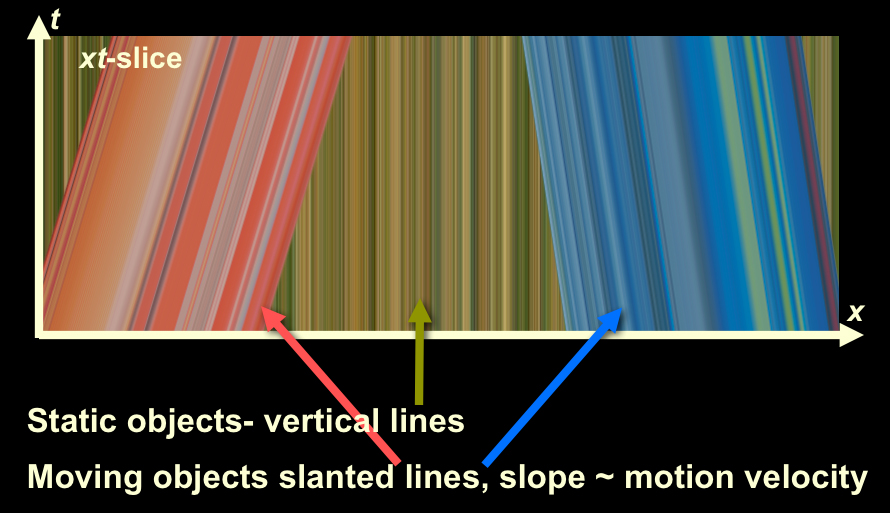
\includegraphics[width=0.6\linewidth]{figures/figs3/spacetime.jpg}
%}
%\caption{Top:  image sequence viewed as a space-time volume.  Bottom:
%The slope in a space-time plot indicates change in x per change in
%time, or the speed.}
%\label{fig:cars12}
%\end{figure}
%
%
%Let's consider the signal itself, Fig.~\ref{fig:cars12}.  Here
%is a 2-d slice of the volumetric video data of 2-d pixel intensities
%observed over time.  In our x-t slice we notice what we learn in
%elementary geometry classes:  the slope of the constant-intensity
%lines, change in time per change in x, indicate the speed of the
%observed pixels.  (This identification assumes constant pixel
%intensities over time).   So identifying the {\em speed} of objects in the
%image is equivalent to finding the {\em orientation} of structures in the
%spatio-temporal volume.  (In the full 3-d video volume, the 3-d
%orientation of constant pixel values indicates the {\em velocity} of
%motion).


%
%
%The fact that we find such space-time filters in neurophysiological
%studies of mammalian visual systems suggests that we may use such
%filter outputs in our own visual systems.  Let's look at a visual
%demonstration which addresses that question.  
%
%Consider a square wave.  From Fourier
%analysis, we know we can synthesize it from a sum of odd harmonics, as
%shown in the equation.  Each frequency comes in with an amplitude of
%$\frac{1}{\omega}$, where $\omega = 2 \pi f$ is its spatial frequency.  
%\begin{equation}
%x_{\mbox{square}}(t) = \frac{4}{\pi}(\sin(2 \pi f t) + \{frac{1}{3}
%\sin(6 \pi f t) + \frac{1}{5} \sin (10 \pi f t) + \hdots)
%\end{equation}
%
%
%Consider the following signal over time:  a square wave, translating
%$\frac{1}{4}$ cycle each frame of a movie.  The signal in space-time
%would look something like this.
%
%What are the different Fourier components of the square wave doing in
%this movie?  The fundamental sine wave has the same frequency as the
%square wave itself, so it, too, is jumping by $\frac{1}{4}$ of a cycle
%(or $90^\circ$) each frame.
%
%The next harmonic, $\frac{1}{3} \sin(3 \omega t)$ jumps by 
%$270^\circ$ each frame, or, equivalently, by $-90^\circ$.  It is
%aliased and, viewed in isolation, would appear to be moving in the
%other direction.
%
%What if we make a``fluted square wave'' signal, the same as
%the original square wave, but with the fundamental sinusoid, 
%$\sin(\omega t)$, subtracted out?  The signal would look like this, in
%space-time.
%
%\begin{figure}
%\centerline{
%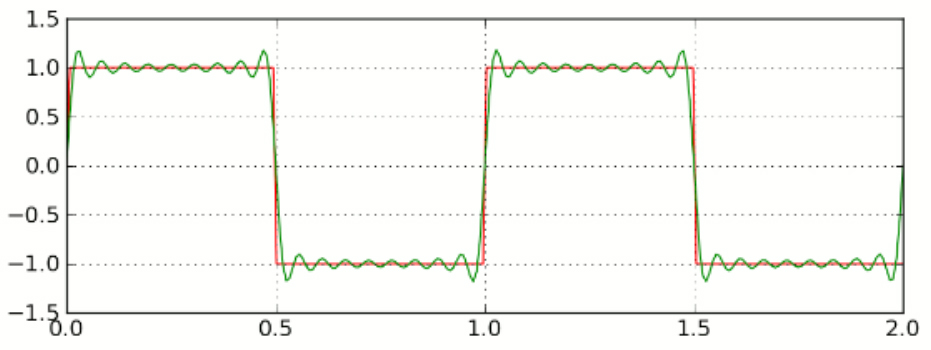
\includegraphics[width=0.8\linewidth]{figures/figs3/sinsquare.jpg}
%}
%\caption{approximation of square wave with sinusoids}
%\label{fig:squaresin}
%\end{figure}
%
%The question is, how would we perceive it moving?  The fluted square
%wave signal is really moving to the left, as the original sine wave
%was.  But the dominant sinusoidal component 
%(which is $\frac{1}{3} \sin(3 \omega t)$, after we remove the
%fundamental from the square wave), viewed in isolation, is moving to
%the right.
%
%\begin{figure}
%\centerline{
%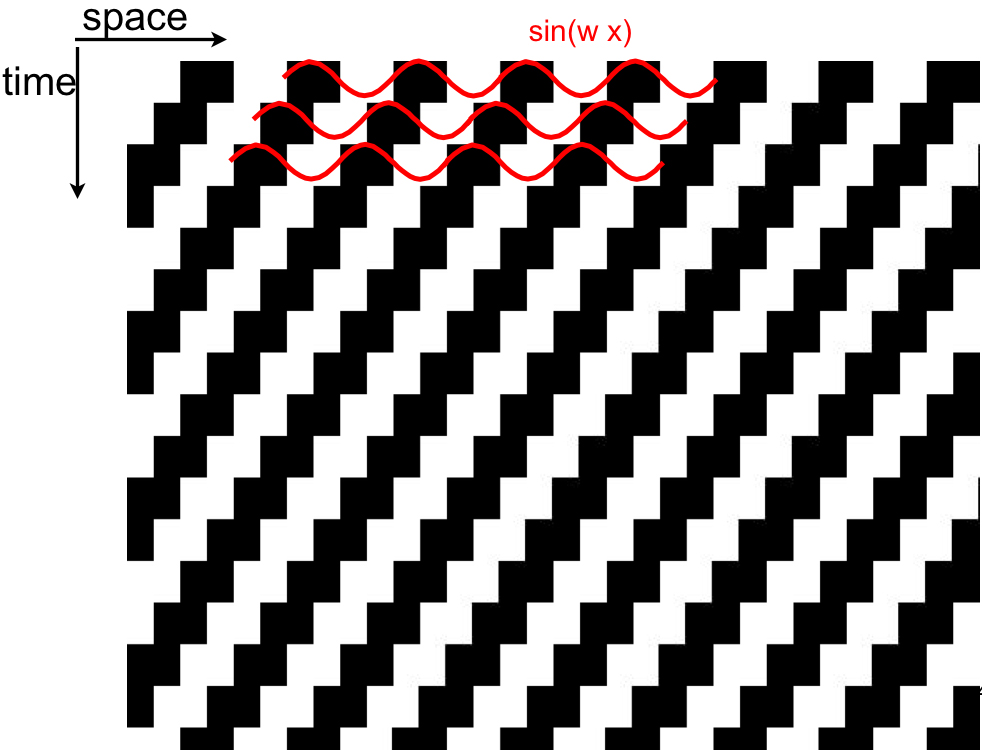
\includegraphics[width=0.6\linewidth]{figures/figs3/squaremotion.jpg}
%}
%\centerline{
%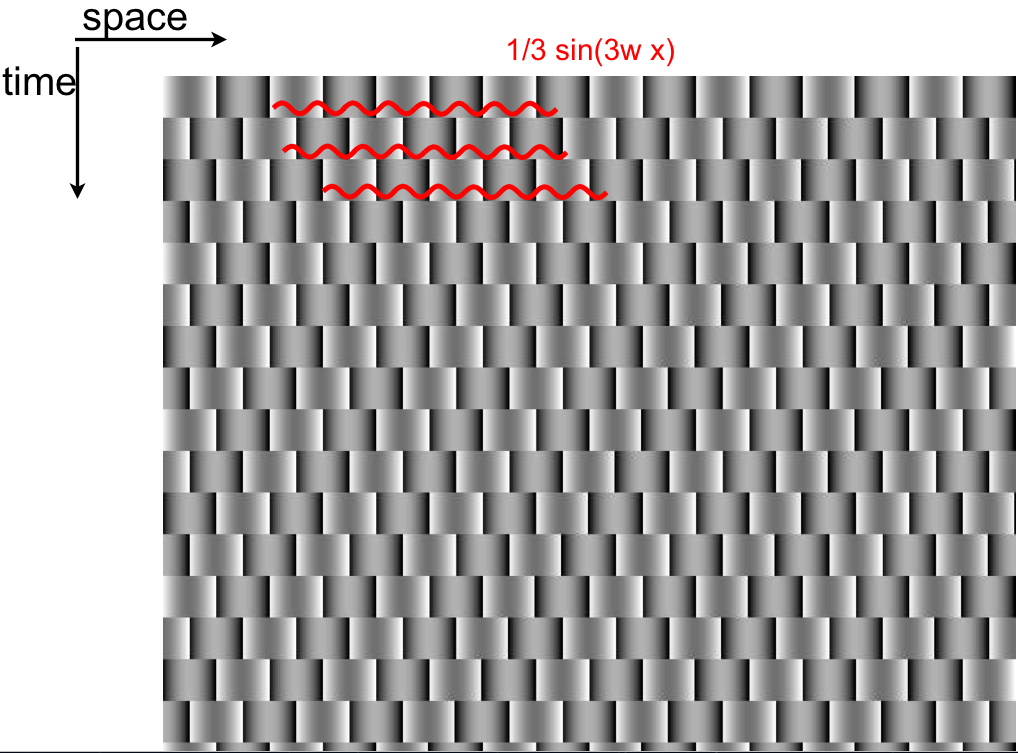
\includegraphics[width=0.6\linewidth]{figures/figs3/flutemotion.jpg}
%}
%\caption{motions}
%\label{fig:motions}
%\end{figure}
%
%
%So will we perceive the signal as an integral whole, and perceive it
%to be moving to the left?  Or will we perceive it as if through a
%federation of oriented filters, each one telling us, for the spatial
%frequency it is tuned to, what is the speed and direction with the
%most motion energy?  Will the visual system choose signal integrity,
%where it has to assimilate all the motion energy filter responses into
%a coherent story describing them all?  Or will it choose computational
%expedience and just listen to the spatio-temporal energy response that
%shouts the loudest?
%
%If we run the experiment, we find  the answer.  The visual
%system seems to take the easy (fast?) way out in this case, and signals
%to us which motion energy filter is responding the strongest:  the
%fluted square wave stimulus appears to be moving to the right.
%
%The quadrature pair motion energy filters, while very simple, are
%powerful enough to perform processing that mimics what a system as
%sophisticated as the human visual system does in some circumstances.
%
%
%\subsection{Motion magnification}
%
%This is an example of dealing with motion signals using filter-based approaches. There is no explicit measurement of motion per se: this method does not explicitly measures velocities.
%
%\begin{figure}
%\centerline{
%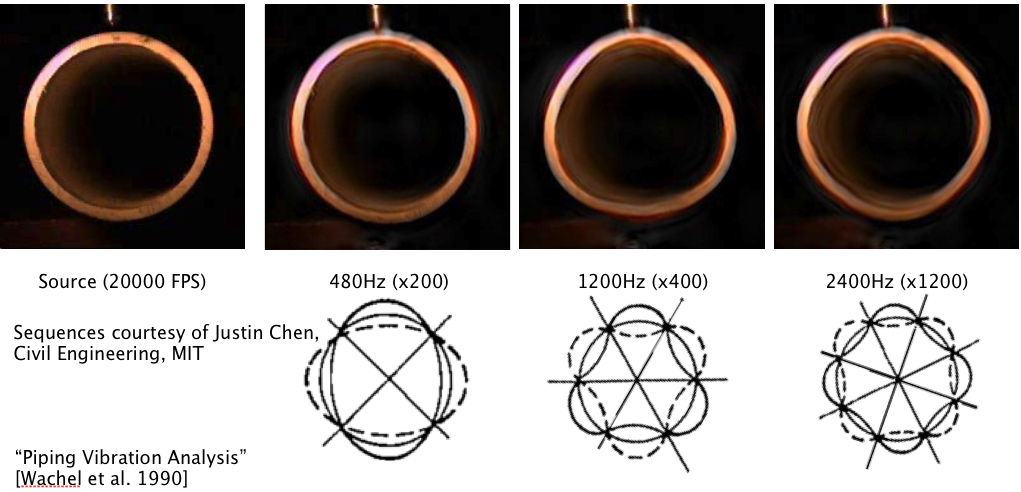
\includegraphics[width=0.8\linewidth]{figures/figs3/pipes.jpg}
%}
%\caption{Still frames of motion magnification output of high-speed
%  video of PVC pipe being struck by a hammer.
%}
%\label{fig:pipes}
%\end{figure}
%
%


%\subsection{The iris code}
%
%\begin{figure}
%\centerline{
%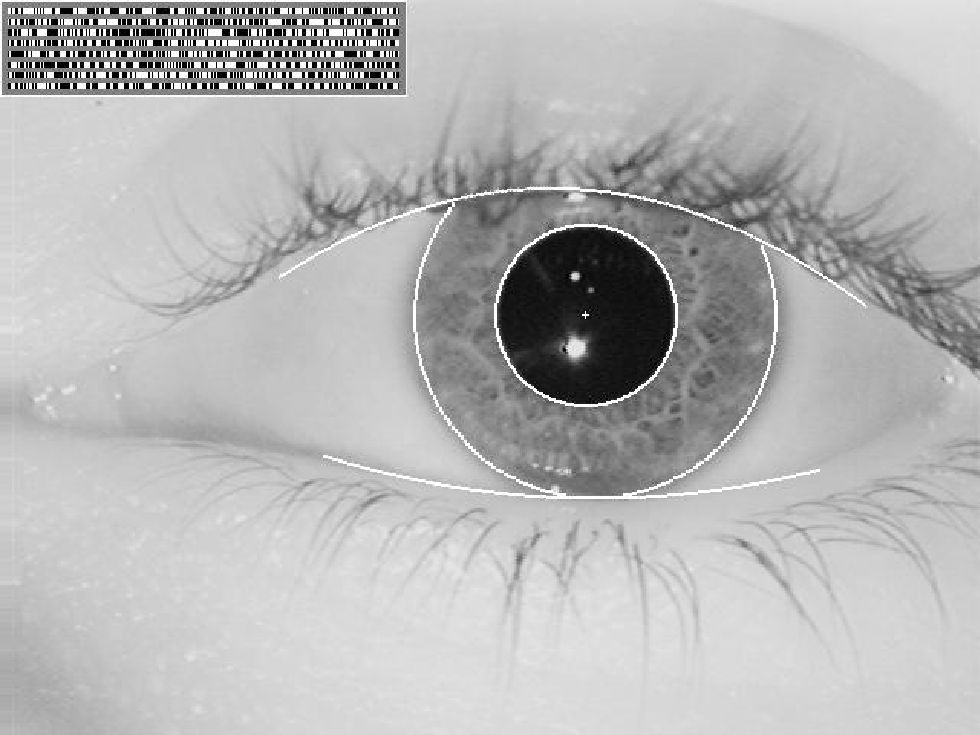
\includegraphics[width=0.4\linewidth]{figures/figs3/daugman1.pdf} 
%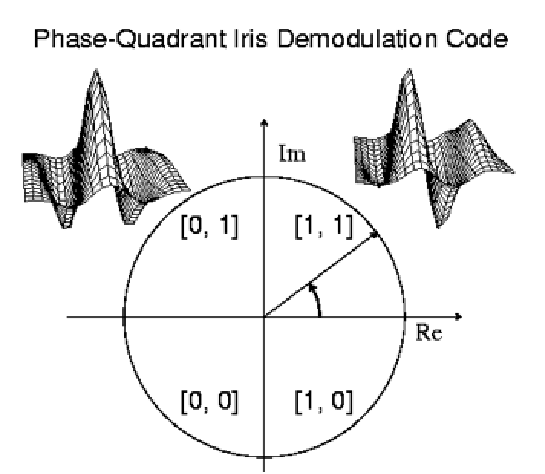
\includegraphics[width=0.4\linewidth]{figures/figs3/daugman2.pdf} 
%}
%\caption{Daugman} 
%\label{fig:daugman}
%\end{figure}
%
%Gabor filters (and indeed, quadrature pair filters in general)
%are useful for many things.   One use they've been put to is in
%quantifying the random textures of the human iris, developed by John
%Daugman, at Cambridge University.   The goal is to
%find a texture descriptor that is invariant to the various 
%conditions under which one might acquire an image of an eye.  The iris
%code measures the relative phase of a Gabor filter pair and quantifies
%that measurement into one of 4 bins (slide 119).  Of course, the
%filters must be aligned with the features of the eye, and
%concentrically oriented around the eye.  The result is a
%high-dimensional code for an individual's iris.  This code is able to
%ascertain identity with very high certainty (and immune to any issues
%with identical twins, because their irises develop under unique random
%processes).
%
%
%
\section{Concluding remarks}
\reviewcomment{To be written.}
